\part{Diffuse lighting}
\frame{\partpage}

\begin{frame}{Diffuse lighting}
	\pause
	\begin{columns}
		\begin{column}{0.33\textwidth}
			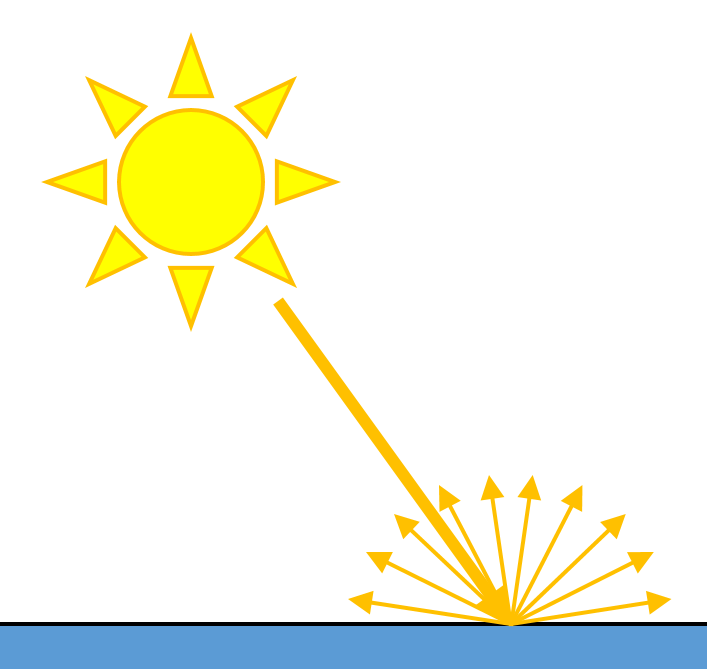
\includegraphics[width=\textwidth]{diffuse_1}
		\end{column}
		\begin{column}{0.65\textwidth}
			When light hits a ``''rough surface, it is \textbf{scattered equally in all directions}
		\end{column}
	\end{columns}
	\pause
	\begin{columns}
		\begin{column}{0.65\textwidth}
			The amount of light hitting the surface depends on the \textbf{angle} between the surface and the light source
		\end{column}
		\begin{column}{0.33\textwidth}
			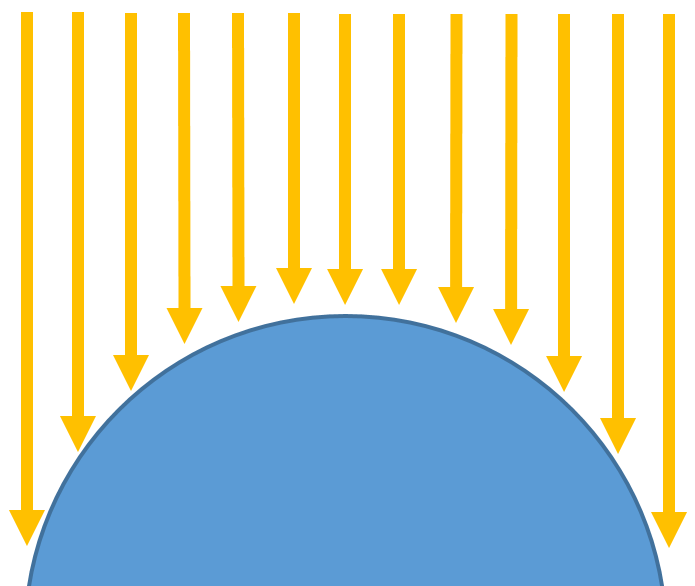
\includegraphics[width=\textwidth]{diffuse_2}
		\end{column}
	\end{columns}
\end{frame}

\begin{frame}{Diffuse lighting formula}
	\begin{columns}
		\begin{column}{0.25\textwidth}
			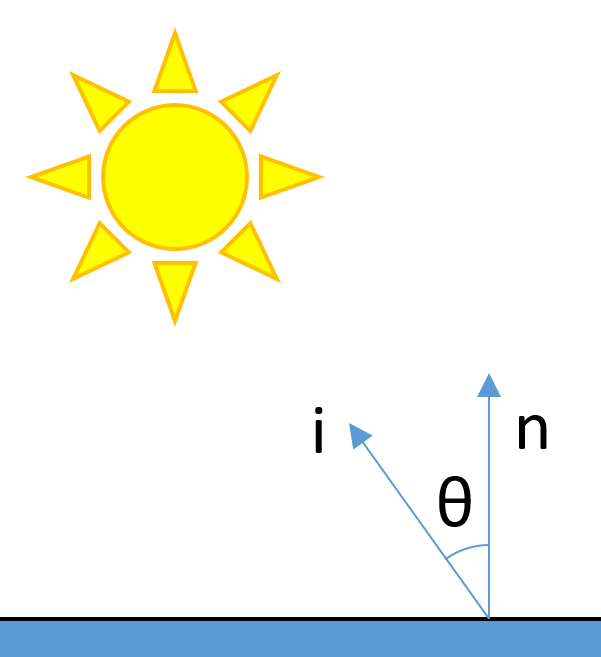
\includegraphics[width=\textwidth]{diffuse_angle}
		\end{column}
		\begin{column}{0.73\textwidth}
			\begin{itemize}
				\pause\item Light intensity is proportional to the \textbf{cosine} of the angle between the \textbf{light direction} and the \textbf{surface normal}
				\pause\item Let $n$ be the normal, and $i$ be a unit vector pointing towards the light source
				\pause\item Light intensity is proportional to
					$\cos \theta = n \cdot i$
				\pause\item If the surface is \textbf{pointing away} from the light source, we get $\theta > \frac{\pi}{2}$ so $\cos \theta < 0$ ---
					in this case we \textbf{clamp} the answer to $0$
			\end{itemize}
		\end{column}
	\end{columns}
\end{frame}

\begin{frame}{Light direction and intensity}
	\begin{itemize}
		\pause\item For a \textbf{distant} light source (e.g.\ the sun),
			direction and intensity are \textbf{constant}
		\pause\item For a \textbf{point} light source (e.g.\ a lightbulb):
			\begin{itemize}
				\pause\item Direction is calculated by subtracting the light position from the fragment position
				\pause\item Intensity obeys an \textbf{inverse square law}: if the distance between the fragment and the light source is $d$,
					then the light intensity is $\frac{1}{d^2}$
			\end{itemize}
	\end{itemize}
\end{frame}

\begin{frame}{Specular lighting}
	\pause
	\begin{columns}
		\begin{column}{0.33\textwidth}
			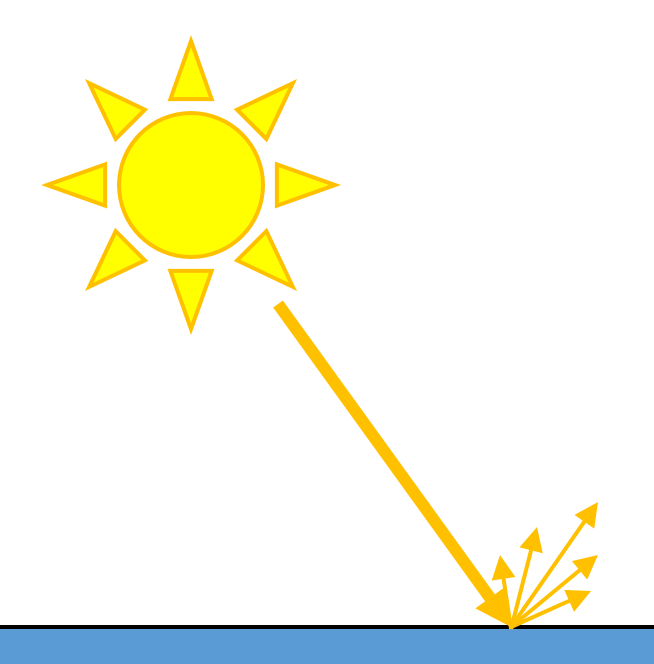
\includegraphics[width=\textwidth]{specular_1}
		\end{column}
		\begin{column}{0.65\textwidth}
			When light hits a ``smooth'' surface, it is \textbf{reflected} across a narrow range of angles
		\end{column}
	\end{columns}
\end{frame}

\begin{frame}{Specular lighting formula}
	\begin{columns}
		\begin{column}{0.33\textwidth}
			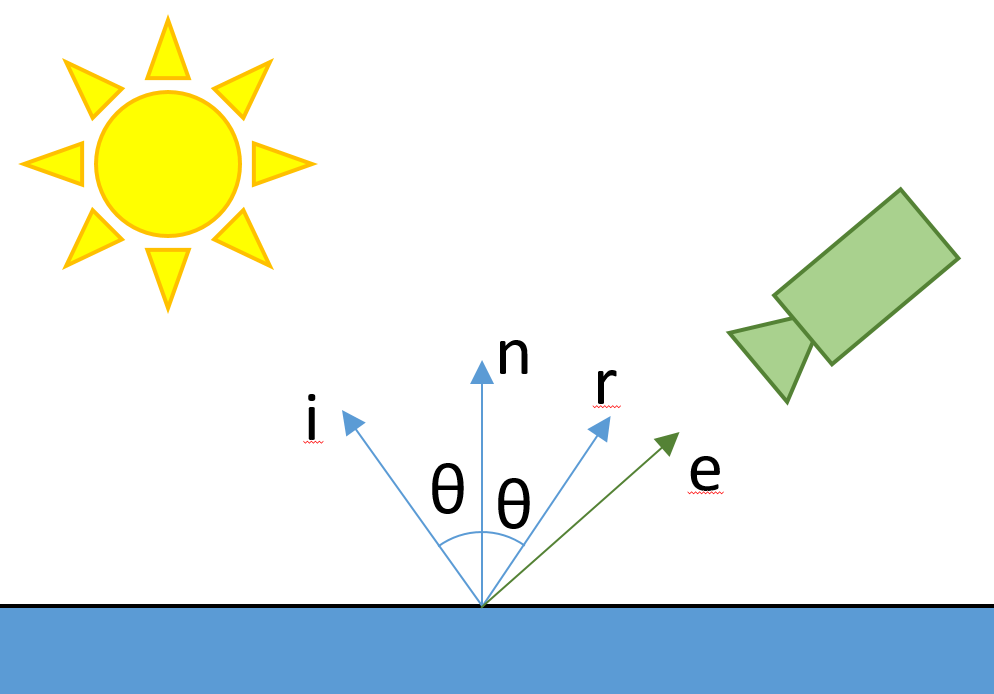
\includegraphics[width=\textwidth]{specular_angle}
		\end{column}
		\begin{column}{0.65\textwidth}
			\begin{itemize}
				\pause\item Let $r$ be the reflection angle (can be calculated in GLSL by \lstinline[language=GLSL]{reflect(-i, n)})
				\pause\item $e$ is a unit vector pointing from the surface towards the camera
			\end{itemize}
		\end{column}
	\end{columns}
	\begin{itemize}
		\pause\item Specular light intensity is proportional to
		$$ \operatorname{clamp}(e \cdot r)^s $$
		where $s$ is a ``shininess'' parameter, and $\operatorname{clamp}(x)$ clamps its argument between $0$ and $1$
	\end{itemize}
\end{frame}

